\documentclass[11pt]{article}
\usepackage{graphicx}
\usepackage[bookmarks=true]{hyperref}
\usepackage{bookmark}
\usepackage{hyperref}
\usepackage{float}
\usepackage{wrapfig}

\usepackage{array}
\newcolumntype{L}[1]{>{\raggedright\let\newline\\\arraybackslash\hspace{0pt}}m{#1}}
\newcolumntype{C}[1]{>{\centering\let\newline\\\arraybackslash\hspace{0pt}}m{#1}}
\newcolumntype{R}[1]{>{\raggedleft\let\newline\\\arraybackslash\hspace{0pt}}m{#1}}

\setlength{\parindent}{0pt}

\begin{document}

\setcounter{tocdepth}{3}
\setcounter{secnumdepth}{5}
\tableofcontents

\newpage
\section{Interface}


\section{Current Interface}
\subsection{Linphone interface}
When a Linphone user opens the application, he/she is greeted and interacts with the following interface:
\begin{itemize}
\item	Light shades of blue/grey, dark grey and orange are used as a colour scheme
\item	The user options are located at the bottom of the screen, represented by ‘self-explanatory’ symbols with an accompanying label.
\item	The user can navigate between these options depending on the needed functionality.
\end{itemize}

\subsection{Chat interface}
The current default interface for a chat between two Linphone users consists of:
\begin{itemize}
\item	A plain blue/grey background
\item	The name of the contact to which the user is currently chatting to is displayed at the top of the chat along with their profile picture.
\centerline{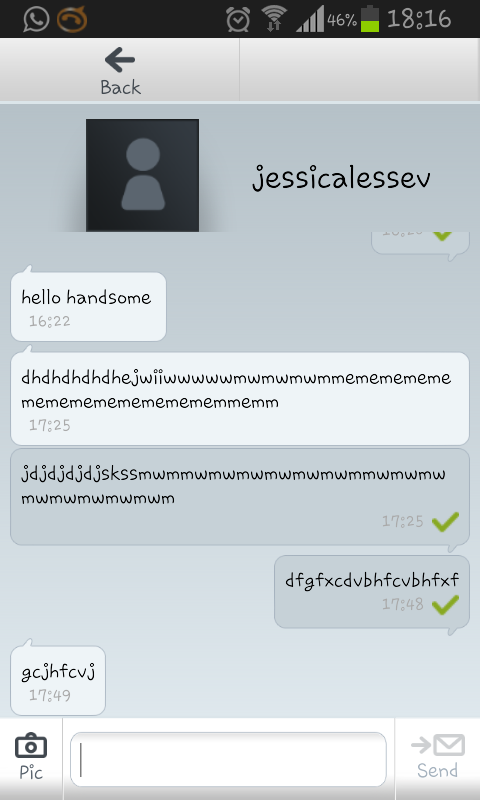
\includegraphics[width=100px]{screen.png}}
\item	Speech bubbles to represent messages
\subitem	Each speech bubble is either left or right aligned depending on whether it is a the users sent message or the users received message.
\subitem	- A received message appears to be left aligned
\subitem	- A message sent by the user appears to be right aligned
\subitem	- All Speech bubbles representing received messages are represented by a light shade of blue
\subitem	- All speech bubbles representing the users’ sent messages are represented by a darker shade of blue.
\item	A yellow arrow represents a sending message
\item	A green tick represents a sent and delivered message
\item	A red cross symbolizes a message that cannot be sent and thus not delivered
\item	When the contact to which the user is chatting to types, the line “Remote is writing…” appears at the bottom of the chat screen

\end{itemize}

\subsection{Potential upgrades and changes to Current interface}
When looking at the current interface that Linphone consists of, from a programmer’s perspective, there are some immediate user interface issues that are noted and that can be changed to accommodate the user better. However after comparing several social networking services, such as Skype, Whatsapp, iMessage, BBM etc, many patterns and standards were identified, answering to layout, presentation, and access to functions and options. To further assist with decision making and changes to be made to the user interface, several users were asked to play around with the application and suggest what they like and do not like about the interface, as well as any additional features and changes that could be made to the interface.\\\\
Applying these noted patterns and standards along with the feedback collected from the few users, the following changes to the interface seem plausible: \\\\
Starting from left to right, looking at each screen/ option located on the bottom of the menu on the Linphone application:
\\ 
\textbf{History Screen}
\begin{itemize}
\item On the top of the screen it is unclear which option is selected between "All" and "Missed" calls. To fix this issue the slider, to indicate the selected option, should be changed to highlight the currently selected option and possibly dim out the unselected option.
\end{itemize}

\textbf{Contacts Screen}
\begin{itemize}
\item On the top of the screen it is unclear which option is selected between "All" and "SIP" contacts. To fix this issue the slider, to indicate the selected option, should be changed to highlight the currently selected option and possibly dim out the unselected option.

\item On the right to the text box, where one would type to search for a contact, the clear button appears as a small white cross in a red circle. This is so even if the user has not typed anything in the search box. The red circle should appear grey or a faded colour until the user types something in the search box after which the circle can return to its original red colour. 

\item When one is typing in the search bar the text as entered should appear to be left-aligned.
\end{itemize}

\textbf{Main/Dial Screen}
\begin{itemize}
\item No noticeable interface problems appear on this menu option.
\end{itemize}

\textbf{Chat Screen}
\begin{itemize}
\item	When one selects the text box to search for a chat the ‘placeholder’ should disappear and the cursor should be left-aligned.

\item When one is typing in the search bar the text as entered should appear to be left-aligned.

\item On the right to the text box, where one would type to search for a chat, the clear button appears as a small white cross in a red circle. This is so even if the user has not typed anything in the search box. The red circle should appear grey or a faded colour until the user types something in the search box after which the circle can return to its original red colour. 

\item The spacing between the search bar and the first chat in the list should be increased.

\item The display of each chat in the list should change to the following format:
\subitem The name of the contact should appear on the first line - left-aligned.
\subitem The time stamp of the last received message should appear on the first line - right-aligned.
\subitem The last received or sent message should appear on the second line\\
This will allow for easy location of a chat and easy reading.\\
\end{itemize}
\setlength\parindent{24pt}\textbf{Within a Chat}
\begin{itemize}
\item A	fine line appears to the right of the "Back" option - since there is not other option to the right this line is useless and should be removed and only added if further options are added to the right of the "Back" button.

\item	Add a defined panel/ bar at the top of a chat to represent the contact to which the user is chatting to. 

\item	Left align the contact details such as picture and name.

\item When one selects the keyboard to type a message the contact's name to which they are talking to changes format. This should not occur and the panel should be kept standard as mentioned in the previous point.

\item	Change the colours of the speech bubbles that represent the messages to be more distinguishable to the background.

\subitem	- The default colour of the speech bubble representing a users’ sent message is very similar to the default background colour and thus it is difficult to distinguish the message from the background. Therefore changing the colour of this will allow the messages to stand out and improve visibility of a message.
\subitem 	- The users’ sent messages should be represented by a duller colour to the received messages as the received messages need more focus.

\item	Limit the size of speech bubbles.
\subitem - Speech bubbles representing a users’ sent message should be limited to stretch to 80\% - 90\% of the screen while being right-aligned.
\subitem	- Speech bubbles representing a received message should be limited to stretch to 80\% - 90\% of the screen while being left-aligned. *
\subitem	- This will allow easier distinguishability between sent and received messages when dealing with longer messages.
\subitem	- Improving on the location, direction and size of speech bubbles will provide for a better feedback system.\\
\centerline{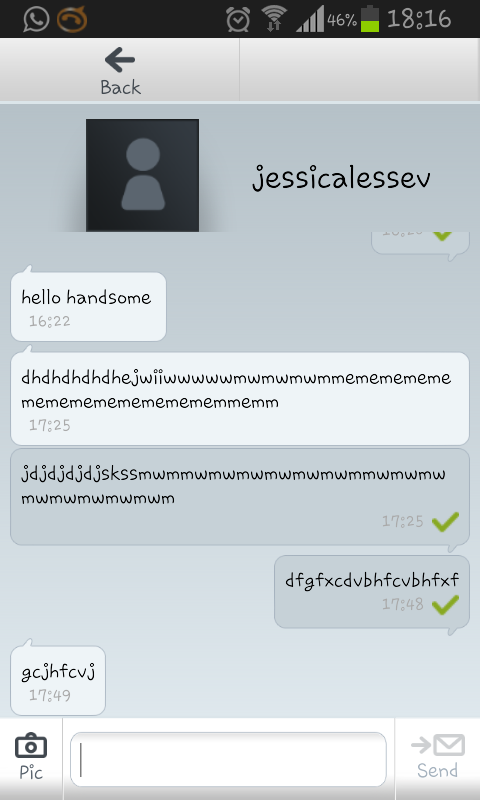
\includegraphics[width=100px]{screen.png}}

\item	The font size of messages should be made larger.

\item	The spacing between words in a messages should be made larger.
\end{itemize}

\textbf{Settings Screen}
\begin{itemize}
\item No noticeable interface problems appear on this menu option.
\end{itemize}

\newpage
\section{Group interface}
\subsection{Design 1}
\centerline{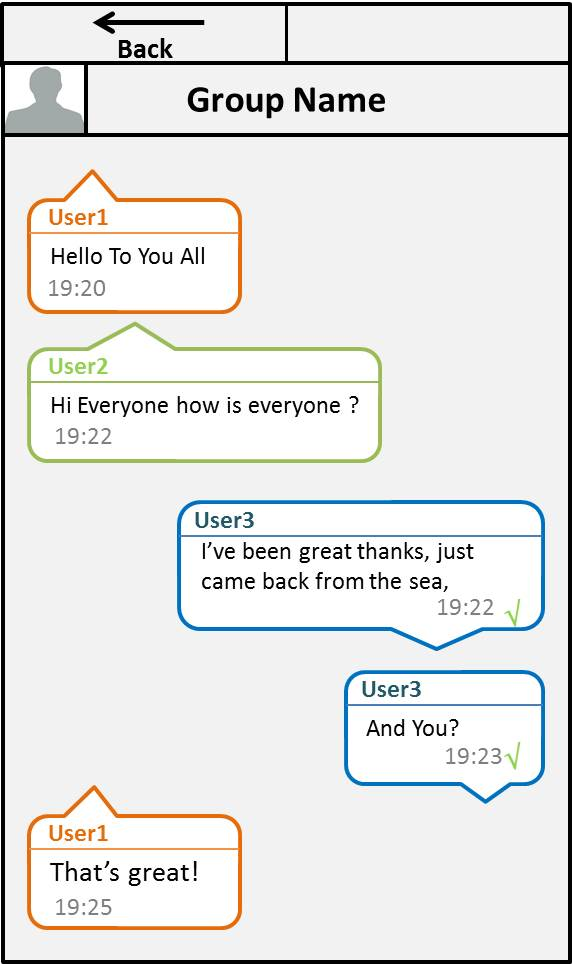
\includegraphics[width=100px]{D01.jpg}}

\textbf{Colours}\\
\begin{itemize}
\item	In order to maintain consistency of design, the same colours chosen to represent the background throughout the application will be used for the user interface for group chats.
\item	Each user will have a randomly assigned colour which will then outline their message speech bubble along with their name in the speech bubble. This will allow better visibility and feedback of messages and their sender.
\item	The colour of the text will remain standard.
\item The timestanp will be a light grey and will appear at the bottom left of the received  messages and on the bottom right of the sent messages.
\item The notification symbols such as the cross and tick to indicate the status of the message will remain their defalt colours.\\
\end{itemize}

\textbf{Font}\\
\begin{itemize}
\item	In order to maintain consistency of design, the font size for each message will be the same as the chosen font size for individual chats.
\item The spacing between text will be adjusted to accomadate reading best.
\end{itemize}

\textbf{Size}\\
\begin{itemize}
\item	The size of the speech bubbles will again be limited to 80\% - 90\% of the screen to delineate the sender of each message. \\
\end{itemize}

\textbf{Speech/Message Bubbles}\\
\begin{itemize}
\item	Each user will have a uniquely coloured bubble to represent their message.
\item	The user sending a message will have their speech bubbles appear on the right such as “User 3” in the above diagram
\item	Each participant in the group, not being the main user will have their message bubbles appear on the left – such as user 1 and 2 in the above diagram.
\item Each message bubble will contain a time stamp that will indicate when the message was sent or received.
\item Sent messages from the user will contain a red cross, yellow or green tick depending on whether the message failed to deliver/send, is sending or sent respectivly.\\
\end{itemize}

\textbf{Participants}\\
\begin{itemize}
\item	When the group name is selected a list of the participants will appear.
\end{itemize}

\newpage
\subsection{Design 2}
\centerline{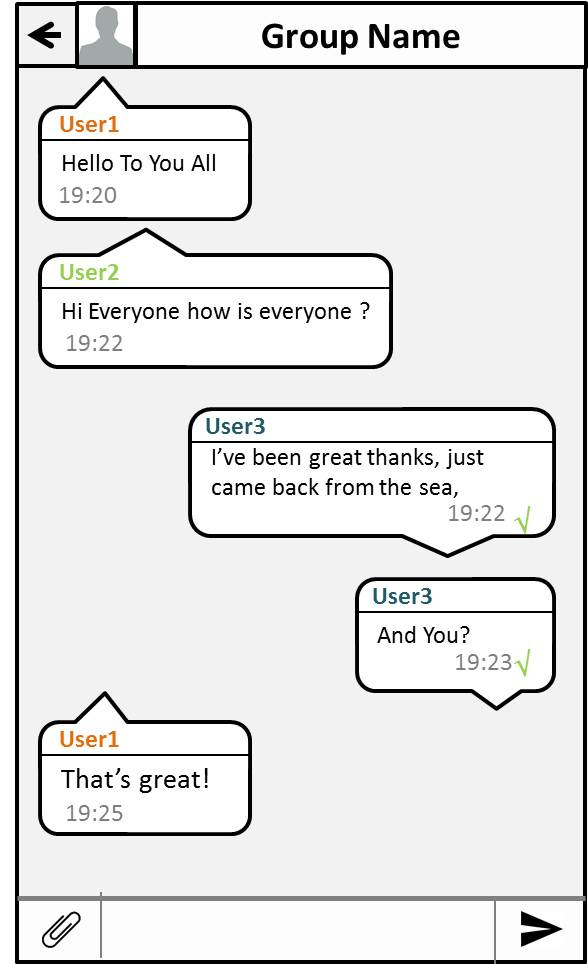
\includegraphics[width=100px]{Final.jpg}}

\textbf{Colours}\\
\begin{itemize}
\item	In order to maintain consistency of design, the same colours chosen to represent the speech bubble and background throughout the application will be used for the user interface for group chats.
\item	Within each speech bubble, each participant’s name will appear in a different colour respectively thus to easily recognize which message came from which participant.
\item	The colour of the text will remain standard.
\item The timestanp will be a light grey and will appear at the bottom left of the received  messages and on the bottom right of the sent messages.
\item The notification symbols such as the cross and tick to indicate the status of the message will remain their defalt colours.\\
\end{itemize}

\textbf{Font}\\
\begin{itemize}
\item	In order to maintain consistency of design, the font size for each message will be the same as the chosen font size for individual chats.
\item The spacing between text will be adjusted to accomadate reading best.
\item	The size of the speech bubbles will again be limited to 80\% - 90\% of the screen to delineate the sender of each message. \\
\end{itemize}

\textbf{Size}\\
\begin{itemize}
\item	In order to maintain consistency of design, the font size for each message will be the same as the chosen font size for individual chats.
\item	The size of the speech bubbles will again be limited to 80\% - 90\% of the screen to delineate the sender of each message. \\
\end{itemize}

\textbf{Speech/Message Bubbles}\\
\begin{itemize}
\item	Each user will have a uniquely coloured name to represent their message.
\item	The user sending a message will have their speech bubbles appear on the right such as “User 3” in the above diagram
\item	Each participant in the group, not being the main user will have their message bubbles appear on the left – such as user 1 and 2 in the above diagram.
\item Each message bubble will contain a time stamp that will indicate when the message was sent or received.
\item Sent messages from the user will contain a red cross, yellow or green tick depending on whether the message failed to deliver/send, is sending or sent respectively.\\
\end{itemize}

\textbf{Space}\\
\begin{itemize}
\item	Moving the group name and picture to appear in the same panel as the "Back" button will allow for more chat space thus more space and less cluttered interface.
\end{itemize}

\textbf{Icons}\\
\begin{itemize}
\item	The send icon will be changed to a paper aeroplane symbol.  
\item Since more than one type of media should be able to be sent as a message, the "Image" icon, to represent sending a picture will be replaced by a paper clip icon with the option to send images and voice notes. 
\item The "Back" button will be replaced by a plain standard arrow to symbolize the "Back" option.  
\end{itemize}

\textbf{Participants}\\
\begin{itemize}
\item	When the group name is selected a list of the participants will appear.
\end{itemize}

\newpage
\subsection{Design 3}
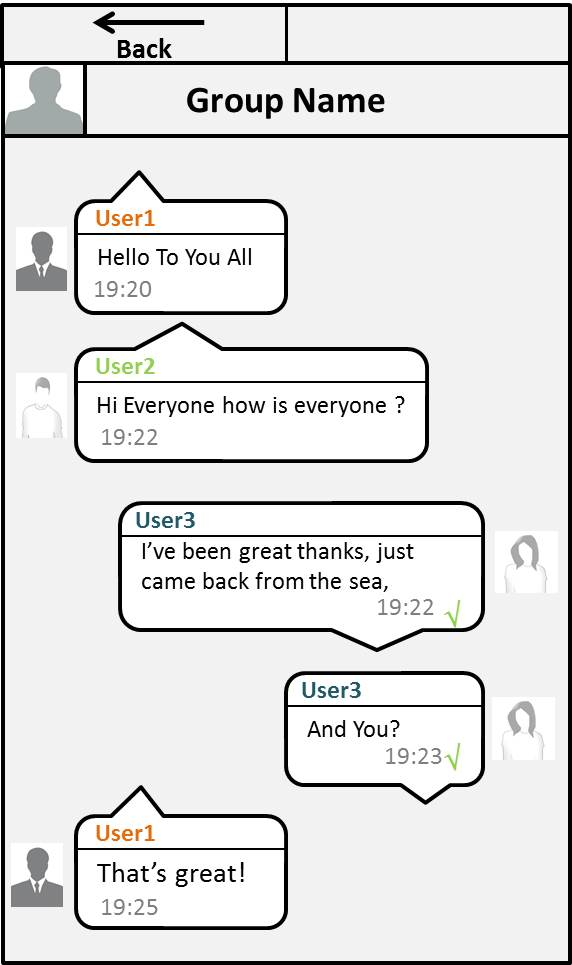
\includegraphics[width=100px]{D03.jpg}  OR  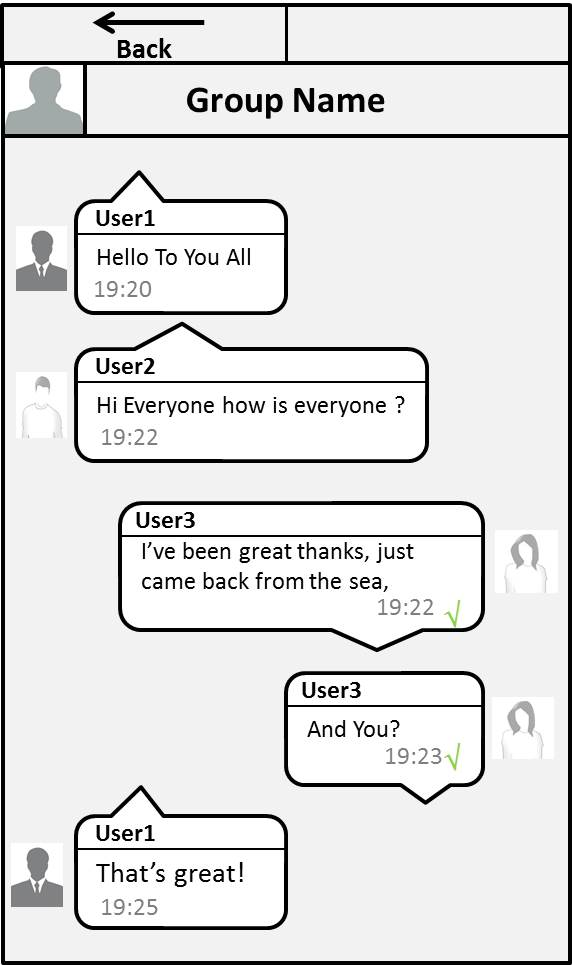
\includegraphics[width=100px]{D03_1.jpg}


\textbf{Colours}\\
\begin{itemize}
\item	In order to maintain consistency of design, the same colours chosen to represent the speech bubble and background throughout the application will be used for the user interface for group chats.
\item	Within each speech bubble, each participant’s name will either appear in a different colour respectively thus to easily recognize which message came from which participant or in a standard black colour depending on the design chosen.
\item	The colour of the text will remain standard.
\item The timestanp will be a light grey and will appear at the bottom left of the received  messages and on the bottom right of the sent messages.
\item The notification symbols such as the cross and tick to indicate the status of the message will remain their defalt colours.\\
\end{itemize}

\textbf{Font}\\
\begin{itemize}
\item	In order to maintain consistency of design, the font size for each message will be the same as the chosen font size for individual chats.
\item The spacing between text will be adjusted to accomadate reading best.
\item	The size of the speech bubbles will again be limited to 80\% - 90\% of the screen to delineate the sender of each message. \\
\end{itemize}

\textbf{Size}\\
\begin{itemize}
\item	In order to maintain consistency of design, the font size for each message will be the same as the chosen font size for individual chats.
\item	The size of the speech bubbles will again be limited to 80\% - 90\% of the screen to delineate the sender of each message. \\
\end{itemize}

\textbf{Speech/Message Bubbles}\\
\begin{itemize}
\item	Each user will have their picture attached to the speech bubble to represent their message.
\item	Each user will have either a uniquely coloured name to represent their message or a black name to represent their message depending on the design chosen.
\item	Attached to each speech bubble will be the users/senders profile picture for easy recognition as to who the message is from.
\item	The user sending a message will have their speech bubbles appear on the right such as “User 3” in the above diagram
\item	Each participant in the group, not being the main user will have their message bubbles appear on the left – such as user 1 and 2 in the above diagram.
\item Each message bubble will contain a time stamp that will indicate when the message was sent or received.
\item Sent messages from the user will contain a red cross, yellow or green tick depending on whether the message failed to deliver/send, is sending or sent respectivly.\\
\end{itemize}

\textbf{Participants}\\
\begin{itemize}
\item	When the group name is selected a list of the participants will appear.
\end{itemize}

\newpage
\subsection{Design 4}
\centerline{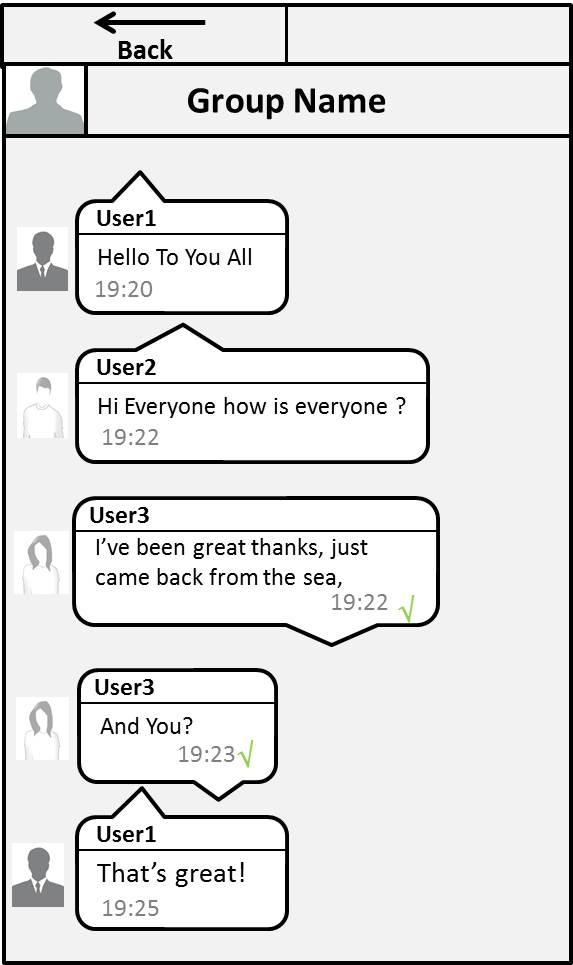
\includegraphics[width=100px]{D04.jpg}}

\textbf{Colours}\\
\begin{itemize}
\item	In order to maintain consistency of design, the same colours chosen to represent the speech bubble and background throughout the application will be used for the user interface for group chats.
\item	The colour of the text will remain standard.
\item The timestanp will be a light grey and will appear at the bottom left of the received  messages and on the bottom right of the sent messages.
\item The notification symbols such as the cross and tick to indicate the status of the message will remain their defalt colours.\\
\end{itemize}

\textbf{Font}\\
\begin{itemize}
\item	In order to maintain consistency of design, the font size for each message will be the same as the chosen font size for individual chats.
\item The spacing between text will be adjusted to accomadate reading best.
\item	The size of the speech bubbles will again be limited to 80\% - 90\% of the screen to delineate the sender of each message. \\
\end{itemize}

\textbf{Size}\\
\begin{itemize}
\item	In order to maintain consistency of design, the font size for each message will be the same as the chosen font size for individual chats.
\item	The size of the speech bubbles will all be limited to the full width of the screen as all the speech bubble will be left-aligned.\\
\end{itemize}

\textbf{Speech/Message Bubbles}\\
\begin{itemize}
\item	All speech bubbles will be left-aligned thus bringing across a neater look and feel
\item	Attached to each speech bubble will be the users/senders profile picture for easy recognition as to who the message is from.
\item Each message bubble will contain a time stamp that will indicate when the message was sent or received.
\item Sent messages from the user will contain a red cross, yellow or green tick depending on whether the message failed to deliver/send, is sending or sent respectivly.\\
\end{itemize}

\textbf{Participants}\\
\begin{itemize}
\item	When the group name is selected a list of the participants will appear.
\end{itemize}

\newpage
\section{Group Chat Information}
\centerline{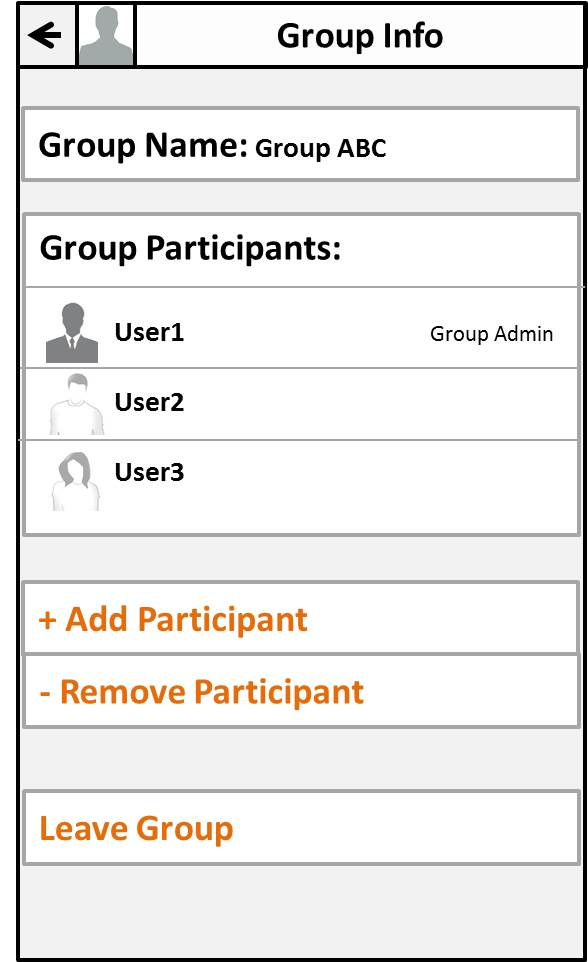
\includegraphics[width=100px]{SettingF.jpg}}

\textbf{Colours}\\
\begin{itemize}
\item	In order to maintain consistency of design, the same colours chosen to represent the background throughout the application will be used for the user interface for group chats.
\item	The colour of the text will remain standard. Text that is important or selectable will be highlighted with a colour to make it noticeable - the default colour is orange. 	\\
\end{itemize}

\textbf{Font}\\
\begin{itemize}
\item	In order to maintain consistency of design, the font size for each message will be the same as the chosen font size for individual chats.
\item The spacing between text will be adjusted to accommodate reading best.\\
\end{itemize}

\textbf{Space}\\
\begin{itemize}
\item	Moving the group name and picture to appear in the same panel as the "Back" button will allow for more chat space thus more space and less cluttered interface.
\end{itemize}

\textbf{Icons}\\
\begin{itemize}
\item	"+" Will be used to symbolize adding a participant to the group.  
\item "-" Will be used to symbolize removing a participant from the group.
\item The "Back" button will be replaced by a plain standard arrow to symbolize the "Back" option.  
\end{itemize}

\textbf{Options Possible}\\
\begin{itemize}
\item	Add Participants: Selecting this option should open the contats page where one can select contacts to add to the group.
\item 	Remove Participants: Selecting this option should open the list of participants in the group where one can select contacts to remove from the group.
\item Leave Group: Selecting this option will cause the user to leave the group and no longer receive messages from the specific group.\\
\end{itemize}


\newpage

\subsubsection{Group Chat Creation}
\begin{figure}[H]
\centering
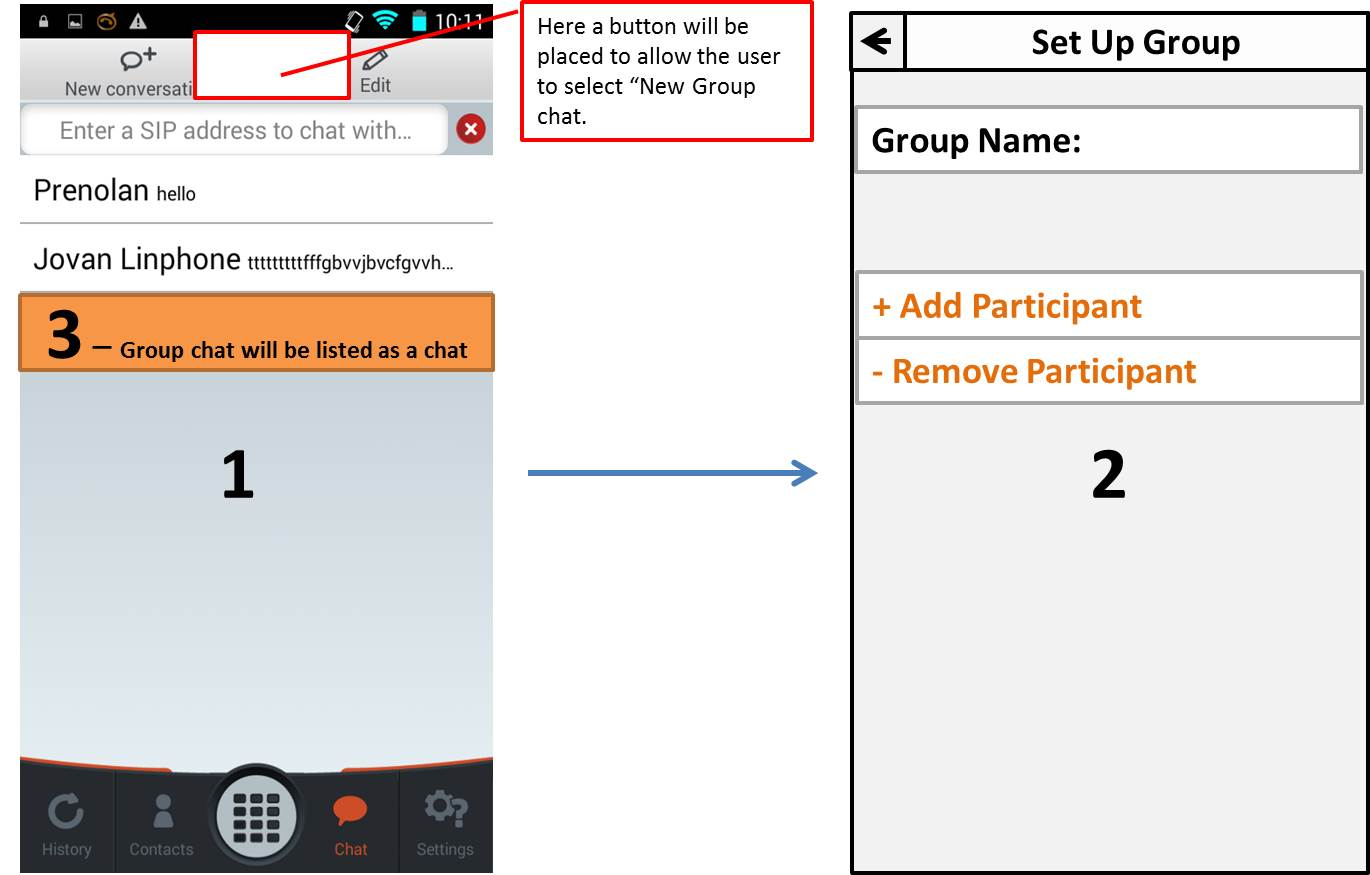
\includegraphics[width=3in]{CG.jpg}
\caption[Create Group Chat]{This diagram shows how the group chat will be created.}
\label{cd-cg}
\end{figure}

\paragraph{Colours}
\begin{itemize}
\item	In order to maintain consistency of design, the same colours chosen to represent the background throughout the application will be used for the user interface for group chat creation option.
\item	The colour of the text will remain standard. Text that is important or selectable will be highlighted with a colour to make it noticeable - the default colour is orange. 	\\
\end{itemize}

\paragraph{Font}
\begin{itemize}
\item	In order to maintain consistency of design, the font size for each message will be the same as the chosen font size for the rest of the application.
\item The spacing between text will be adjusted to accommodate best reading.\\
\end{itemize}

\paragraph{Icons}
\begin{itemize}
\item	"+" Will be used to symbolize adding a participant to the group.  
\item "-" Will be used to symbolize removing a participant from the group.
\item The "Back" button will be replaced by a plain standard arrow to symbolize the "Back" option. 
\item A paper clip represents attaching a media file, in this case a profile picture.  
\end{itemize}

\paragraph{Options Possible}
\begin{itemize}
\item Type group name.
\item Select or browse phone gallery to set a profile picture for the group.
\item	Add Participants: Selecting this option will open the contacts page where one can select contacts to add to the group.
\item 	Remove Participants: Selecting this option will open the list of participants in the group where one can select contacts to remove from the group.
\end{itemize}

\paragraph{Process}
\begin{enumerate}
\item The user will, in the "Chat" interface select the option "New Group Chat" - number 1 in the diagram.
\item The Group chat set up page will be displayed. Here the user will fill in the necessary information needed in order to create a group chat - number 2 in the diagram.
\item Finally, once the group chat has been created, the Group chat name will appear in the list of the user's chats and will be able to be selected and used - number 3 in the diagram.
\end{enumerate}


\end{document}